\documentclass[a4paper,oneside,11pt,english]{report}

\usepackage{graphicx}
\usepackage{indentfirst}
\usepackage{color}
\usepackage{setspace}
\usepackage[pdftex,pdfpagelabels,bookmarks,hyperindex,hyperfigures]{hyperref}
\usepackage{bookmark}
\usepackage[paper=a4paper,top=1in,bottom=1in,right=1in,left=1.5in]{geometry}



\begin{document}
%------------------------------------TITLE PAGE------------------------------------------------------------------------------------------------
\pagenumbering{roman}  %Roman page no.s for Front page 


\begin{titlepage}
	\newgeometry{margin=.5in}
	{
		\begin{center}
			
\includegraphics[width=.2\linewidth]{logo/walchand.jpg}\\[.5cm]
			\textbf{\LARGE Walchand College of Engineering, Sangli }\\
			\textbf {(An Autonomous Institute)}\\[.5cm]
			\textbf {\Large Department\\ of\\ Computer Science and Engineering}\\[1.5cm]
			{ \large \textbf{ A  Seminar Report\\ on} }\\[.5cm]
			\textbf{\Large Automated Shopping Marts : A look at the future stores}\\[2cm]
			%%%%%%%%%%%%%%%%%%%%%%
			\iffalse
			\textit \large{Submitted in partial fulfillment of the requirements for the award of degree of
				}\\[1cm]
			\textbf{BACHELOR OF TECHNOLOGY\\ IN \\COMPUTER SCIENCE AND ENGINEERING
				}\\[1cm]
			\fi
			%%%%%%%%%%%%%%%%%%%%%%
			\large  {Submitted by}\\[1cm]
			%	\end{center}
			{\setlength{\tabcolsep}{30pt}
				\renewcommand{\arraystretch}{1.5}
				\begin{tabular}{ll}
					\large{Vaibhav Ananda Kumbhar } & \large{2012BCS057} 
					%& \large\textbf{vkumbhar94@gmail.com}  
					\\
					\large {Akshay Shirish Habbu }&\large{2012BCS095}
					% & \large\textbf{akshayhabbu4@gmail.com}
					\\
					\large{Machchindra Sanjay Pol} & \large{2012BCS091}
					% &  \large\textbf{machchindrapol@gmail.com}
					\\
				\end{tabular}\\[1.5cm]
			}
			\large  {Under the Guidance\\ of}\\[1cm]
			\Large \textbf{ Dr. P. J. Kulkarni  }\\[1cm]
			
			%	\begin{center}
			\vfill
			\large \textbf{2015-2016 }\\[.4cm]
		\end{center}
	}
\end{titlepage}





%-------------------------------------------CERTIFICATE-----------------------------------------------------------------------------
\newpage
%\begin{titlepage}
%\begin{stretchbox}
{	
	\newgeometry{top=1in,bottom=1in,right=2in,left=1in}
	\linespread{2}
	
	\begin{center}
		
\includegraphics[width=.2\linewidth]{logo/walchand.jpg}\\[.5cm]
		\textbf{\Large Walchand College of Engineering, Sangli }\\
		\textbf {(An Autonomous Institute)}\\[.5cm]
		\textbf {\LARGE Department of Computer Science and Engineering}\\[1cm]
		{\color{blue}\huge\textbf{{\underline{CERTIFICATE}}}}\\[1cm]
	\end{center}
	\linespread{1.6}
	\par \large Certified that the seminar work entitled \textbf{Automated Shopping Marts : A look at the future stores}  ​ is bonafied work carried out by \textbf{Vaibhav Kumbhar (2012BCS057), Akshay Habbu (2012BCS095) and Machchindra Pol (2012BCS091)} , ​ in partial fulfillment of the completion of $ 7^{th} $ Semester Bachelor of Computer Science and Engineering of Walchand college of Engineering, Sangli, during the year 2015-2016. It is certified that all the suggestions indicated for internal assessment have been incorporated in the ​report. The Seminar report has been approved as it ​satisfies the academic requirements in respect of seminar work prescribed for the Semester. \\[2cm]
	%\vfill
	\vspace{6cm}
	\begin{minipage}{.5\linewidth}
		\begin{flushleft}
			\textbf{Guide}\\
			\textbf{Dr. P. J. Kulkarni}\\
		\end{flushleft}
	\end{minipage}
	\begin{minipage}{.5\linewidth}
		\begin{flushright}
			
			\textbf{H.O.D}\\
			\textbf{Dr. B. F. Momin}\\
		\end{flushright}
	\end{minipage}
	
}


\restoregeometry
\doublespacing

\iffalse
\begin{abstract}
	AJKAHKDJADHK
\end{abstract}
\fi


\tableofcontents
\listoffigures
\clearpage

\pagenumbering{arabic} %Arabic for chapters
\chapter{Introduction}
\section{The Idea}
{
	\iffalse
	Imagine a completely automated Shopping-Mart.  When you enter the store, there are, generally, no employees to help you.  At most times, the only people in the store are registered customers. Entering customers are greeted by an automated greeting assistant. Most consumers bring their shopping lists with them from home on their PDAs.  They choose an intelligent shopping cart which is equipped with a PSA- a Personal Shopping Assistant. If a consumer cannot find what he is looking for, help is just a button away.  Consumers could press the Instant Help button on their intelligent shopping cart. Consumers are responsible for the checkout process however they can pay online or they can just pay amount on counter directly. 
	\fi
	"Imagine a completely automated Shopping-Mart. When you enter the store, there are, generally, no employees to help you. At most times, the only people in the store are registered customers."
	\par The basic idea behind this project and above statement was to make use of the simple technologies around us and bring on the change that will help improving the lifestyle. The idea revolves around automating most of the processes of shopping inside the mega stores. Such that it would not only help in easing out the process but also reduces human resources required for it. Making use of technologies around us is sufficient to implement this project. we talk about assisting the user about the path he'll need to follow during shopping can be nothing but a simple query to the perfect database of the store and even describing each product detail is a query to the database of products table.

	\par Managing a cart which scans the products on the go, can be implemented by proper integration of devices like bar-code scanner and LCD screen (small) using raspberry pi kit.

	\par We are always surrounded by the different technologies, making right integration of them can turn such massive ideas into reality.

}
\chapter{Application}
\section{Typical User Experience}

	\subsection{Entry}
	\par Entry to the unmanned Shopping-Mart is through a biometric security system.  Registered customers enter the store by simply pressing their thumb on a reader.  Readers are available at two heights to accommodate various ages and profiles.  A two-door entry system ensures that only authorized visitors might enter.  Video and still images are taken of every entering customer for security purposes.   
	\par New visitors are directed to kiosks outside the store for the registration process.  Here, they have to fill out a short form, provide a major credit card and have a picture taken.  Then, they provide a thumbprint to authenticate their identity and they are instantaneously registered. 
	
	
	
	
	\subsection{Intelligent Shopping Cart }
	
	Most consumers bring their shopping lists with them from home on their PDAs.  They choose an intelligent shopping cart which is equipped with a PSA- a Personal Shopping Assistant.  Consumers can transfer their shopping list from a PDA to a PSA in an instant.  If a consumer does not have a PDA, s/he can simply upload the list using a Web interface before coming to the store.  Alternatively, a consumer might type in their shopping list directly on to a PSA. 
	\par The PSA assists consumers by- a) retrieving specials and promotions for items that are similar to what the consumer picked and b) providing them with a map that minimizes their walking time in the store.  The map points out the location of the item by aisle, shelf and location- e.g. end of aisle 23, middle shelf.     
	\par If the PSA does not recognize something, it will say so.  It provides a Spellcheck program to minimize spelling errors.  The PSA remembers old lists created by the consumer allowing it to serve up information speedily. 
	
	
	\subsection{Help Finding an Item}
	If a consumer cannot find what he is looking for, help is just a button away.  Consumers could press the Instant Help button on their intelligent shopping cart.  The Instant Help button connects consumers to a call center where trained care representatives provide targeted assistance.  Globally dispersed call centers allow for instant assistance- the company promises help within 10 rings or 10\% off on the entire purchase.  Care representatives can interact with the PSA on the intelligent shopping cart to accurately locate and map items. 
	
	
	\subsection{Checking Out}
	Consumers are responsible for the checkout process.  However, the burden on the consumer is reduced due to intelligent shopping cart technology. 
	\par All items in the store are RFID-tagged.  When the consumer approaches the checking line, the intelligent shopping cart provides a total on the PSA by reading the RFID tags.   
	\par Consumers can check out using the option to pay bycash, credit or debit card.   
	
\iffalse	
\section{Special Situations}

	\subsection{Expensive Items }
	Items that are small and expensive are frequent targets of shoplifters.  e.g. Ipods.  Such items are placed in a special enclosure.  To enter this enclosure, consumers will have to re-authenticate- i.e., provide their biometric id one more time to enter.  This allows the store to minimize damages due to shoplifting. 
\fi


\chapter{Analysis}

\section{Technical Requirements}

	\subsection{Hardware Requirements}
	\begin{enumerate}
		\item {
			\textbf{Raspberry Pi}
			\par The Embedded chip which controls the entire operation. Raspberry Pi  has the ability to interact with the outside world.\\
			\begin{figure}[ht]
				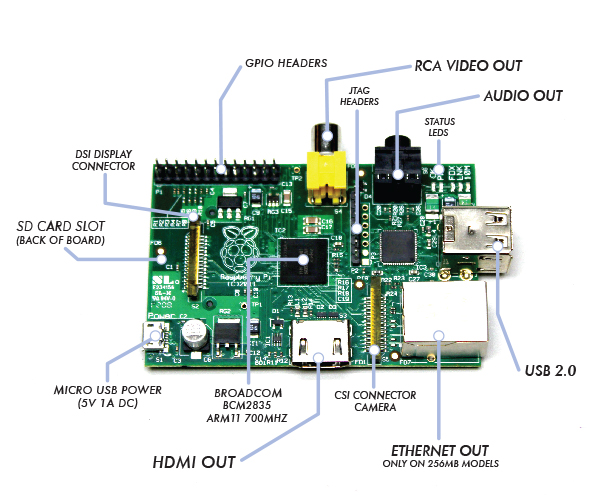
\includegraphics[width=\linewidth]{images/raspberry-pi.jpg}
				\caption{Raspberry Pi}
			\end{figure}
		}
		\item {
			\textbf{4" Touch Screen LCD monitor}
			\par A mini 4 inch Touch Screen LCD monitor is integrated with the Raspberry Pi used to interact with customer.
		}
		\item {
			\textbf{2 Barcode Scanners Or Webcams}
			\par Two Barcode Scanners or webcams are connected and installed with the Raspberry Pi Embedded Chip to read the  product codes. 
		}
		\item {
			\textbf{100V battery}
			\par A 100V battery kit powers the Raspberry pi and the LCD monitor through adapter which gives 5v DC supply to the devices.
		}
		\item {
			\textbf{3 biometric thumb scanners}
			\par 3 biometric thumb scanners required at entrance and registration kiosks.
		}
	\end{enumerate}
	\subsection{Software Requirements}
		\begin{enumerate}
			\item {
				\textbf{Sql Database Server}
				\par Sql Database server ( Microsoft Sql Server) which provides higher storage capacity, security to data. Availability of data helps us to store customer credentials like passwords, debit card information.
			}
			\item {
				\textbf{Raspbian OS}
				\par An ARM based Operating System to be installed on raspberry pi to handle whole assembly of a cart. Raspberry pi is device having 512MB to 1GB RAM. Linux Distributions are able to run on it. Raspbian OS is ARMv6 based RISC(Reduced Instruction Set Computer) OS . As python is default language for rasbian OS, Ease to write code modules.
			}
		\end{enumerate}
\section{Connectivity}
	\subsection{Cart to Central Server connection}
	\par Cart Assembly is connected to the central server by Wifi. Wifi is secured with the WPA authentication so intruders won't get connectivity with wifi.\\
	\begin{figure}[ht]
		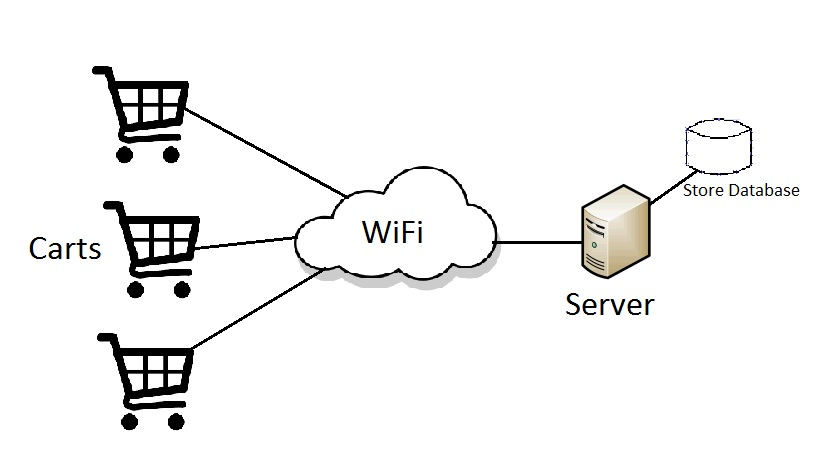
\includegraphics[width=\linewidth]{images/connection1.jpg}
		\caption{Schematic Connectivity}
	\end{figure}
	\subsection{Cart Integration}
		\par Cart is having raspberry pi placed on it. Touch screen connected to raspberry pi. 2 scanners are connected to Raspberry pi. the whole devices are powered by 5v DC Supply.
		\par The integrated cart will look like:\\ 
		\begin{figure}[ht!]
			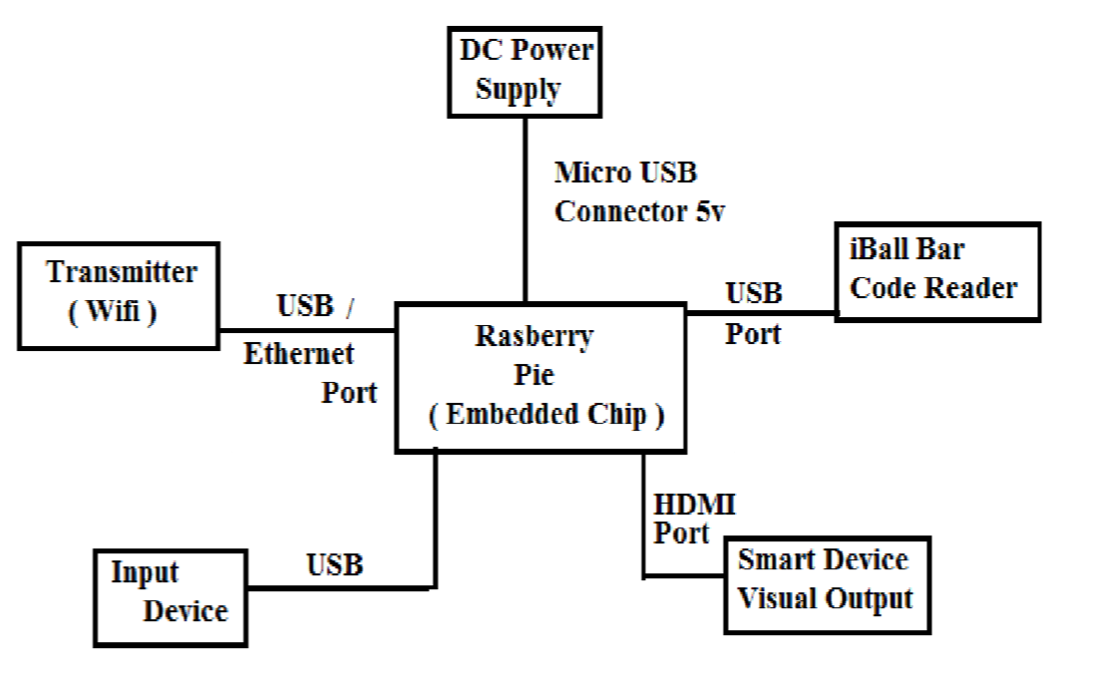
\includegraphics[width=\linewidth]{images/innercart.png}
			\caption{Connectivity of devices on cart}
		\end{figure}
\section{Data Storage}
	\subsection{OLTP Transactions}
		\par Sql Server provides Online transactions on database. The product data and customer is need to be transfer securely. 
		The Security is provided by sql server.
		\par Security Features of Sql Server as follows:\\
			\begin{enumerate}
				\item {
					\textbf{Authentication in SQL Server}
					\par Describes logins and authentication in SQL Server and provides links to additional resources.
				}
				\item {
					\textbf{Authorization and Permissions in SQL 	Server}
					\par Describes granting permissions using the principle of least privilege and provides links to additional resources.
				}
				\item {
					\textbf{Data Encryption in SQL Server}
					\par Describes data encryption options in SQL Server and provides links to additional resources.
				}
			\end{enumerate}
	\subsection{SSH and Secure Copy}
		\par SSH uses the RSA encryption algorithm to generate public and private keys, making intrusion extremely difficult.
		Since SSH is a remote login protocol, It is used to manage cart assembly when it fails or not working. by SSH we can control the raspberry pi device.
		Protocol SCP (Secure Copy) run on top of SSH, we can use it  to transfer data from one cart to another or with server.
		SSH supports one time log in. This means that once cart assembly connects to the central system. we dont need to reintialize it again and again.
	\subsection{View of Data}
		\par The logical view of data consists of product infomation , it's brands, Sale Information. \\Schema for Inventory of products.\\
		\begin{figure}[ht]
			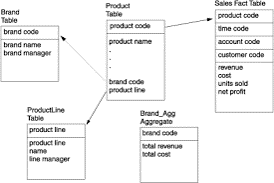
\includegraphics[width=\linewidth]{images/Schema.png}
			\caption {Schema of Inventory of products}
		\end{figure}
		
	\subsection{Functional Block Diagram of Cart}
	\par Cart is having two barcode scanners placed on top of it. When barcode on product scanned and validated then the inlet tray is opened and customer can drop it in cart. When customers wants to remove product from cart then when he requests, the tray opens and barcode scans and that product is removed from bill inventory.
	\begin{figure}[ht]
		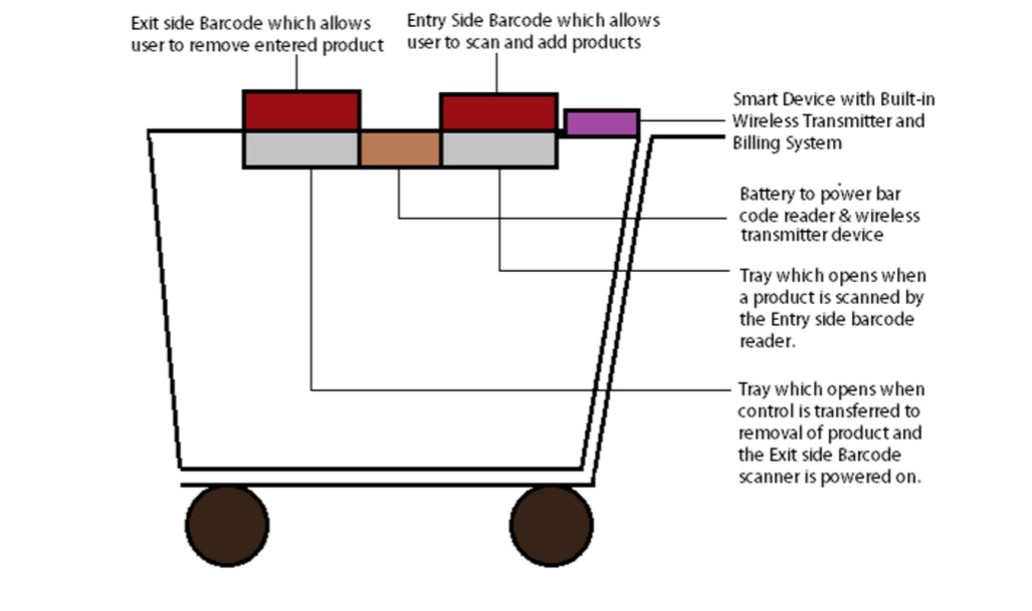
\includegraphics[width=\linewidth]{images/cartlook.jpg}
		\caption{Functional Block Diagram}
	\end{figure}
	
\chapter{Conclusion and Advantages}
\section[To Company]{Why is this better for the Company? }

	The company comes out ahead by-  
	\begin{itemize}
		\item  Greater profit margins by reduction of labor cost.
		\item  Greater information on consumers allows the company to predict demand and personalize offerings and service. 
		\item  Better consumer service attracts more consumers.   
	\end{itemize}
\section[To Consumer]{Why is this better for the Consumer? }
	The consumer benefits from- 
	\begin{itemize}
		 \item Improved service due to greater control over process. 
		 \item  Improved consumer security through the use of technology. 
		 \item  Greater post-sales information through the shopping analysis service.    
	\end{itemize}
\iffalse
\chapter{Conclusion}
	By integrating all the assembly, we can look to the future marts.
\fi


\iffalse
\chapter{References}
	\begin{enumerate}
		\item {
			 The Automated Wal-Mart- A Thought Experiment$_{-Sandeep Krishnamurthy} $
		}
		
		\item {
			Smart Shopping Cart for Automated Billing Purpose using Wireless Sensor Networks-$ _{Udita Gangwal, Sanchita Roy, Jyotsna Bapat}$
		}
		
		\item {
			Automated Shopping Trolley for Super Market Billing System- $ _{S. Sainath, K. Surender, V. Vikram Arvind Final Year,  Department of Computer Science and Engineering Hindustan University Chennai, India  }$
		}
	\end{enumerate}
\fi
\clearpage
\addcontentsline{toc}{chapter}{Bibliography}
\bibliographystyle{IEEEtran}
\bibliography{references}
\nocite{*}
\end{document}
